%======================================================================
%	
%	 __  __       _         ______ _ _      
%	|  \/  |     (_)       |  ____(_) |     
%	| \  / | __ _ _ _ __   | |__   _| | ___ 
%	| |\/| |/ _` | | '_ \  |  __| | | |/ _ \
%	| |  | | (_| | | | | | | |    | | |  __/
%	|_|  |_|\__,_|_|_| |_| |_|    |_|_|\___|
%
%----------------------------------------------------------------------
% Descripton : Main File to compose the resulting PDF
%======================================================================
%\pdfobjcompresslevel=0
\pdfminorversion=7
\pdfinclusioncopyfonts=1
\documentclass[
				ngerman             % neue deutsche Rechtschreibung
				,a4paper            % Papiergrösse
				%,twoside            % Zweiseitiger Druck (rechts/links)
				% ,10pt             % Schriftgrösse
				,11pt
				% ,12pt
				,pdftex
				%  ,disable         % Todo-Markierungen auschalten
				,notitlepage		% Thanks abstract... preventing it from removing pageNumber
				]{report}

%————————————————————————————————————————————————————————————————————————————
%					Import aller Konfigurationen
%————————————————————————————————————————————————————————————————————————————
\usepackage{./config/DHBW/bericht}
\usepackage{./config/PaketeProjektarbeit} % <- spezifische Pakete für die Projektarbeit
\usepackage{./config/Pakete}
\usepackage{./config/Befehle}
\usepackage{./config/Layout}
\usepackage{./config/Styles}
%Wenn PDF/A-1B gewünscht .. Achtung am besten nochmal mit veraPDF testen!
\usepackage{./config/PDFStandard}

%————————————————————————————————————————————————————————————————————————————
%					Variablen deklarieren
%————————————————————————————————————————————————————————————————————————————
%======================================================================
%	
%	__      __        _       _     _            
%	\ \    / /       (_)     | |   | |           
%	 \ \  / /_ _ _ __ _  __ _| |__ | | ___ _ __  
%	  \ \/ / _` | '__| |/ _` | '_ \| |/ _ \ '_ \ 
%	   \  / (_| | |  | | (_| | |_) | |  __/ | | |
%	    \/ \__,_|_|  |_|\__,_|_.__/|_|\___|_| |_|
%
%----------------------------------------------------------------------
% Descripton : Variables
%======================================================================

\newboolean{DEBUG}
\newboolean{BERICHTE}
\newboolean{SPERRVERMERK}
\newboolean{CHANGELOG}
\newboolean{VORWORT}
\newboolean{ABSTRACT}
\newboolean{DANKSAGUNG}
\newboolean{WATERMARK}
\newboolean{INDEX}
\newboolean{TRENNSTRICHE}
\newboolean{ERKLAERUNG}
\newboolean{DOKUMENTENVERZEICHNIS}
\newboolean{DATEIVERZEICHNIS}
\newboolean{LITERATURVERWEIS}
\newboolean{DIGITALE-UNTERSCHRIFT}
\newboolean{DIGITAL-SIGN-AREA}

%————————————————————————————————————————————————————————————————————————————
%					Informationen ausfüllen
%————————————————————————————————————————————————————————————————————————————
%======================================================================
%	
%	_____        __                           _   _             
%  |_   _|      / _|                         | | (_)            
%	 | |  _ __ | |_ ___  _ __ _ __ ___   __ _| |_ _  ___  _ __  
%    | | | '_ \|  _/ _ \| '__| '_ ` _ \ / _` | __| |/ _ \| '_ \ 
%	_| |_| | | | || (_) | |  | | | | | | (_| | |_| | (_) | | | |
%  |_____|_| |_|_| \___/|_|  |_| |_| |_|\__,_|\__|_|\___/|_| |_|
%
%----------------------------------------------------------------------
% Descripton : File with all Information about the Document
%======================================================================

\newcommand{\Autor}{Kristin Agne}
\newcommand{\MatrikelNummer}{9262783}
\newcommand{\Kursbezeichnung}{TINF19B4}

\newcommand{\FirmenLogoDeckblatt}{
\includegraphics[width=5cm]{./config/layout/seriephant}}

% Falls es kein Firmenlogo gibt:
%  \newcommand{\FirmenLogoDeckblatt}{}

\newcommand{\BetreuerDHBW}{Mirko Dostmann}

%%%%%%%%%%%%%%%%%%%%%%%%%%%%%%%%%%%%%%%%%%%%%%%%%%%%%%%%%%%%%%%%%%%%%%%%%%%%%%%%%%%%%

% Wird auf dem Deckblatt und in der Erklärung benutzt:
%\newcommand{\Was}{Projekt-/Studien-/Bachelorarbeit}
%\newcommand{\Was}{Projektrarbeit}
%\newcommand{\Was}{Studienarbeit}
%\newcommand{\Was}{Bachleorarbeit}
\newcommand{\Was}{Programmentwurf}

%%%%%%%%%%%%%%%%%%%%%%%%%%%%%%%%%%%%%%%%%%%%%%%%%%%%%%%%%%%%%%%%%%%%%%%%%%%%%%%%%%%%%

\newcommand{\Titel}{Projektdokumentation Seriephant}
\newcommand{\AbgabeDatum}{16. Mai 2022}

\newcommand{\Dauer}{5. \& 6. Semester}

% \newcommand{\Abschluss}{Bachelor of Engineering}
\newcommand{\Abschluss}{Bachelor of Science}

\newcommand{\Studiengang}{Informatik / Informationstechnik}
% \newcommand{\Studiengang}{Informatik / Angewandte Informatik}
%======================================================================
%	 _    _                                 __ 
%	| |  | |                               / _|
%	| |__| |_   _ _ __   ___ _ __ _ __ ___| |_ 
%	|  __  | | | | '_ \ / _ \ '__| '__/ _ \  _|
%	| |  | | |_| | |_) |  __/ |  | | |  __/ |  
%	|_|  |_|\__, | .__/ \___|_|  |_|  \___|_|  
%		     __/ | |                           
%		    |___/|_|                           
%
%----------------------------------------------------------------------
% Descripton : Hyperref File for setting PDF Information
%======================================================================

\hypersetup{
	bookmarks=true,
	unicode=false,
	pdftoolbar=true,
	pdfmenubar=true,
	pdffitwindow=false,
	pdfstartview={FitH},
	pdftitle={\Titel},
	pdfauthor={\Autor},
	pdfsubject={\Was},
	pdfcreator={\Autor},
	pdfkeywords={DHBW},
	pdfborderstyle={/S/U/W 1},
	pdfnewwindow=true,
	citebordercolor=LimeGreen,
	filebordercolor=Magenta,
	linkbordercolor=Orange,
	menubordercolor=Orange,
	urlbordercolor=Fuchsia,
	runbordercolor=Orange
}


%————————————————————————————————————————————————————————————————————————————
%					Sonstige Einstellungen
%————————————————————————————————————————————————————————————————————————————
\bibliography{./directories/bibliography}
\loadglsentries{./directories/glossary}
\makeglossaries

%————————————————————————————————————————————————————————————————————————————
%					Einstellungen
%————————————————————————————————————————————————————————————————————————————
% Debug auf true setzen, hierbei wird der Changelog hinzugefügt, und keine Doppelseitenumbrüche gemacht (Zum drucken -> false)
% Bitte zum drucken oben in der Präambel auch auf Doppelseite schalten!
\setboolean{DEBUG}{true}
% Soll eine Erklärung eigefügt werden ?
\setboolean{ERKLAERUNG}{false}
%Soll das Abstract eingefügt werden ?
\setboolean{ABSTRACT}{false}
%Soll ne Trennlinie im Inhaltsverzeichnis eingefügt werden, vor Verzeichnissen, dem Inhalt und dem Anhang
\setboolean{TRENNSTRICHE}{true}
%Setzt ein Watermark
\setboolean{WATERMARK}{false}
%Dokumentenverzeichnis generieren ?

%————————————————————————————————————————————————————————————————————————————
%					Watermark
%————————————————————————————————————————————————————————————————————————————
\ifthenelse{\boolean{WATERMARK}}{\usepackage{draftwatermark}}{}
\ifthenelse{\boolean{WATERMARK}}{\SetWatermarkText{Entwurf}}{}

%————————————————————————————————————————————————————————————————————————————
%									Anfang Dokument
%————————————————————————————————————————————————————————————————————————————
\begin{document}
	% Wer keine Seitenzahlen braucht bis zum TOC einfach das Pagenumbering auf gobble und an der Stelle an der die Seitenzählung beginnen soll roman einfügen
	\pagenumbering{gobble}
	\pagestyle{plain}
	
	%—————————————————————————————————————————————————————————————————————————
	%								Deckseite
	%—————————————————————————————————————————————————————————————————————————
	\begin{titlepage}
		%%%%%%%%%%%%%%%%%%%%%%%%%%%%%%%%%%%%%%%%%%%%%%%%%%%%%%%%%%%%%%%%%%%%%%%%%%%%%%%
%% Descr:       Vorlage für Berichte der DHBW-Karlsruhe, Titlepage
%% Author:      Prof. Dr. Jürgen Vollmer, vollmer@dhbw-karlsruhe.de
%% $Id: erklaerung.tex,v 1.11 2020/03/13 14:24:42 vollmer Exp $
%% -*- coding: utf-8 -*-
%%%%%%%%%%%%%%%%%%%%%%%%%%%%%%%%%%%%%%%%%%%%%%%%%%%%%%%%%%%%%%%%%%%%%%%%%%%%%%%

\begin{center}
	\vspace*{-2cm}
	\FirmenLogoDeckblatt\hfill
\includegraphics[width=5cm]{./config/DHBW/dhbw-logo.png}\\[2cm]
	{\Huge \Titel}\\[1cm]
	{\Huge\scshape \Was}\\[1cm]
	{\large der Vorlesung \hk{\textbf{A}dvanced \textbf{S}oftware \textbf{E}ngineering}}\\[0.5cm]
	{\large an der}\\[0.5cm]
	{\large Dualen Hochschule Baden-Württemberg Karlsruhe}\\[0.5cm]
	{\large von}\\[0.5cm]
	{\large\bfseries \Autor}\\[1cm]
	{\large Abgabedatum \AbgabeDatum}
	\vfill
\end{center}
\begin{tabular}{l@{\hspace{2cm}}l}
	Matrikelnummer	                 	& \MatrikelNummer		\\
	Kurs			         			& \Kursbezeichnung		\\
	Bearbeitungszeitrum					& \Dauer 				\\
	Gutachter der Studienakademie	 	& \BetreuerDHBW			\\
\end{tabular}
	\end{titlepage}

	% Ab hier beginnt die Seitenzählung für den Prefix in kleinen römischen Zahlen
	% Erste Seite nach der Titelseite
	\pagenumbering{roman}
	\setcounter{page}{2}
	\ifthenelse{\boolean{DEBUG}}{}{\cleardoublepage}
	
	
	
	%—————————————————————————————————————————————————————————————————————————
	%								Erklärung
	%—————————————————————————————————————————————————————————————————————————
	\ifthenelse{\boolean{ERKLAERUNG}}{\phantomsection}{}
	\ifthenelse{\boolean{ERKLAERUNG}}{%%%%%%%%%%%%%%%%%%%%%%%%%%%%%%%%%%%%%%%%%%%%%%%%%%%%%%%%%%%%%%%%%%%%%%%%%%%%%%%
%% Descr:       Vorlage für Berichte der DHBW-Karlsruhe, Erklärung
%% Author:      Prof. Dr. Jürgen Vollmer, vollmer@dhbw-karlsruhe.de
%% $Id: erklaerung.tex,v 1.11 2020/03/13 14:24:42 vollmer Exp $
%% -*- coding: utf-8 -*-
%%%%%%%%%%%%%%%%%%%%%%%%%%%%%%%%%%%%%%%%%%%%%%%%%%%%%%%%%%%%%%%%%%%%%%%%%%%%%%%

% In Bachelorarbeiten muss eine schriftliche Erklärung abgegeben werden.
% Hierin bestätigen die Studierenden, dass die Bachelorarbeit, etc.
% selbständig verfasst und sämtliche Quellen und Hilfsmittel angegeben sind. Diese Erklärung
% bildet das zweite Blatt der Arbeit. Der Text dieser Erklärung muss auf einer separaten Seite
% wie unten angegeben lauten.

\newpage
\thispagestyle{empty}
\begin{framed}
\begin{center}
\Large\bfseries Erklärung
\end{center}
\medskip
\noindent
% siehe §5(3) der \enquote{Studien- und Prüfungsordnung DHBW Technik} vom 29.\,9.\,2017 und Anhang 1.1.13
Ich versichere hiermit, dass ich meine \Was \ mit dem Thema:
\enquote{\Titel}
selbstständig verfasst und keine anderen als die angegebenen Quellen und Hilfsmittel benutzt habe. Ich versichere zudem, dass die eingereichte elektronische Fassung mit der gedruckten Fassung übereinstimmt. \\
\vspace{3cm} \\
\ifthenelse{\boolean{DIGITALE-UNTERSCHRIFT}}{\includegraphics[height=1.5\baselineskip]{./zfiles/Signaturen/Ort_Datum} \hfill \includegraphics[height=2\baselineskip]{./zfiles/Signaturen/Signatur} \hspace{0.1cm} \vspace{-0.5cm} \\}{}
\ifthenelse{\boolean{DIGITAL-SIGN-AREA}}{\sigField{Digitale Signatur}{14cm}{2cm}}{}
\ifthenelse{\boolean{DIGITAL-SIGN-AREA}}{\underline{\hspace{14cm}} \\ \hspace{4cm} Digitale Unterschrift}{\underline{\hspace{6cm}}\hfill\underline{\hspace{6cm}} \\ Ort~~~~~~~~~~~~~Datum \hfill Unterschrift\hspace{4cm}}
\end{framed}

%%%%%%%%%%%%%%%%%%%%%%%%%%%%%%%%%%%%%%%%%%%%%%%%%%%%%%%%%%%%%%%%%%%%%%%%%%%%%%%
\endinput
%%%%%%%%%%%%%%%%%%%%%%%%%%%%%%%%%%%%%%%%%%%%%%%%%%%%%%%%%%%%%%%%%%%%%%%%%%%%%%%
}{}
	\ifthenelse{\boolean{ERKLAERUNG}}{\addcontentsline{toc}{chapter}{Erklärung}}{}
	\ifthenelse{\boolean{DEBUG}}{}{\cleardoublepage}
	
	%—————————————————————————————————————————————————————————————————————————
	%								Abstract
	%—————————————————————————————————————————————————————————————————————————
	\ifthenelse{\boolean{ABSTRACT}}{\phantomsection}{}
	\ifthenelse{\boolean{ABSTRACT}}{%%%%%%%%%%%%%%%%%%%%%%%%%%%%%%%%%%%%%%%%%%%%%%%%%%%%%%%%%%%%%%%%%%%%%%%%%%%%%%%
%% Descr:       Vorlage für Berichte der DHBW-Karlsruhe, Abstract
%% Author:      Prof. Dr. Jürgen Vollmer, vollmer@dhbw-karlsruhe.de
%% $Id: abstract.tex,v 1.11 2020/03/13 14:24:42 vollmer Exp $
%% -*- coding: utf-8 -*-
%%%%%%%%%%%%%%%%%%%%%%%%%%%%%%%%%%%%%%%%%%%%%%%%%%%%%%%%%%%%%%%%%%%%%%%%%%%%%%%

\vspace*{5cm}
%\vspace*{\fill}

\begingroup
	\centering
	\begin{abstract}
		\addcontentsline{toc}{chapter}{Zusammenfassung}
		Dieses \LaTeX-Dokument kann als Vorlage für einen Praxis- oder Projektbericht, eine Studien- oder Bachelorarbeit dienen.
		Zusammengestellt von Prof.\,Dr.\,Jürgen Vollmer \email{juergen.vollmer@dhbw-karlsruhe.de}
		\url{https://www.karlsruhe.dhbw.de} modifiziert von Nico Holzhäuser \email{nico.holzhaeuser@abilis.de} \url{https://abilis.de}. \\
		Die jeweils aktuellste Version dieses \LaTeX-Paketes ist immer
		auf der \emph{FAQ-Seite} des Studiengangs Informatik zu finden:
		\url{https://www.karlsruhe.dhbw.de/inf/studienverlauf-organisatorisches.html} $\to$ \emph{Formulare und Vorlagen}.
		\centering Stand \verb+$Date: 2020/09/17 15:07:45 $+
		\centering Stand DHBW \verb+$Date: 2020/03/13 15:07:45 $+
	\end{abstract}
\endgroup

\vspace*{\fill}}{}
	\ifthenelse{\boolean{DEBUG}}{}{\cleardoublepage}
	
	%—————————————————————————————————————————————————————————————————————————
	%							Inhaltsverzeichnis
	%—————————————————————————————————————————————————————————————————————————
	\setcounter{tocdepth}{1}% Allow only \chapter in ToC
	\ifthenelse{\boolean{DEBUG}}{}{\cleardoublepage}
	
	\phantomsection
	\addcontentsline{toc}{chapter}{Inhaltsverzeichnis}
	\tableofcontents           % Inhaltsverzeichnis hier ausgeben
	\ifthenelse{\boolean{DEBUG}}{\newpage}{\cleardoublepage}
	
	\phantomsection
	\listoffigures             % Liste der Abbildungen
	\addcontentsline{toc}{chapter}{Abbildungsverzeichnis}
	\ifthenelse{\boolean{DEBUG}}{\newpage}{\cleardoublepage}
	
%	\phantomsection
%	\lstlistoflistings         % Liste der Codeschnipsel
%	\addcontentsline{toc}{chapter}{Codeverzeichnis}
%	\ifthenelse{\boolean{DEBUG}}{\newpage}{\cleardoublepage}
	
	\phantomsection
	\ifthenelse{\boolean{TRENNSTRICHE}}{\addtocontents{toc}{\protect\mbox{}\protect\hrulefill\par}}{}
	%======================================================================
%                                              
%	    /\                                        
%	   /  \   ___ _ __ ___  _ __  _   _ _ __ ___  
%	  / /\ \ / __| '__/ _ \| '_ \| | | | '_ ` _ \ 
%	 / ____ \ (__| | | (_) | | | | |_| | | | | | |
%	/_/    \_\___|_|  \___/|_| |_|\__, |_| |_| |_|
% 	                              __/ |          
%	                              |___/             
%
%----------------------------------------------------------------------
% Author : Nico Holzhäuser
% Descripton : Cover Page
%======================================================================

\chapter*{Abkürzungsverzeichnis} % chapter*{..} --> keine Nummer, kein "Kapitel"
						         % Nicht ins Inhaltsverzeichnis
\addcontentsline{toc}{chapter}{Abkürzungsverzeichnis}   % Damit das doch ins Inhaltsverzeichnis kommt

% Hier werden die Abkürzungen definiert
% 1-10 nur damit der Abstand default auf diese Länge gesetzt wird
\begin{acronym}[12345678910]
  	%\acro{Name}{Darstellung der Abkürzung}{Langform der Abkürzung}
	\acro{DHBW}[DHBW]{Duale Hochschule Baden-Württemberg}
	\acro{UML}[UML]{Unified Modeling Language}
	\acro{DDD}[DDD]{Domain Driven Design}
	\acro{UL}[UL]{Ubiquitous Language}


	% Folgendes benutzen, wenn der Plural einer Abk. benöigt wird
	% \newacroplural{Name}{Darstellung der Abkürzung}{Langform der Abkürzung}
	\newacroplural{Abk}[Abk-en]{Abkürzungen}

	% Wenn neicht benutzt, erscheint diese Abk. nicht in der Liste
	\acro{NUA}[]{Not Used Acronym}
	
\end{acronym}
 %Acronyms

	\ifthenelse{\boolean{DEBUG}}{\newpage}{\cleardoublepage}
		
	
	%—————————————————————————————————————————————————————————————————————————
	%								Inhalt
	%—————————————————————————————————————————————————————————————————————————
	%Hauptteil normale arabische Zählung, beginnend bei 1 und alten Pagestyle wiederherstellen!
	\pagenumbering{arabic} 
	\setcounter{page}{1}
	\pagestyle{headings} %<- Pagestyle reset 
	
	%%%%%%%%%%%%%%%%%%%%%%%%%%%%%%%%%%%%%%%%%%%%%%%%%%%%%%%%%%%%%%%%%%%%%%%%%%%%%%%
%% Descr:       Vorlage für Berichte der DHBW-Karlsruhe
%% Author:      Prof. Dr. Jürgen Vollmer, vollmer@dhbw-karlsruhe.de
%% Modified :	Kristin Agne, TINF19B4
%% -*- coding: utf-8 -*-
%%%%%%%%%%%%%%%%%%%%%%%%%%%%%%%%%%%%%%%%%%%%%%%%%%%%%%%%%%%%%%%%%%%%%%%%%%%%%%%

\chapter{Domain Driven Design}
\ac{DDD} ist eine Philosophie zur Modellierung komplexer Software. Der Fokus liegt hierbei auf dem präzisen und tiefgreifenden Verständnis der Problemdömane. Desweiteren bietet es Muster, um ein konsistentes, erweiterbares, funktionierendes Modell der Problemdomäne zu entwickeln.

\section{Ubiquitous Language}
Die \ac{UL} ist das wichtigste Konzept des \ac{DDD}. Es bezeichnet die von Domänenexperten und Entwicklern gemeinsam im Projekt verwendete Sprache. Dadurch sollen gleiche Begriffe in der Domäne, sowie in dem Sourcecode, verwendet werden. Durch die \ac{UL} sollen Verständnisschwierigkeiten zwischen Domänenexperten und Entwicklern minimiert werden. Durch \ac{UL} ist der Code näher an der Sprache der Domäne. Als \ac{UL} bezichnet man den Teil des Projektes, der sich von den Entwicklern und den Domänenexperten überschneiden (siehe \cref{a.1.pic}).

\subsection{Analyse}
Die Fachdomäne ist in diesem Projekt sehr überschaubar. Damit in dem Projekt keine Sprachprobleme aufkommen, wurde als Sprache Englisch gewählt, da diese international verständlich ist. Die Fachbegriffe der einzelnen Objekte und deren Bedeutung sowie Attribute wurde im Voraus wie folgt festgelegt:

\subsubsection{Genre}
Unter einem Genre wird eine Kategorie verstanden, die einer Serie zugeordnet werden kann. Diese sind global definiert.
\subsubsection{Actor}
Unter einem Actor versteht man einen Schauspieler. Dies ist eine Person, die in einzelnen Episoden mitspielen kann.
\subsubsection{Serie}
Eine Serie ist eine Fernsehshow, bei der regelmäßig Folgen von Sendungen ausgestrahlt werden.
\subsubsection{Season}
Eine Season stellt eine Staffel von einer Serie dar. Hierbei werden Episoden thematisch gegliedert in Handlungsabschnitte, und alle Folgen werden in zeitlicher Nähe ausgestrahlt.
\subsubsection{Episode}
Eine Episode stellt eine einzelne Folge da, die einer Staffel und somit auch einer Serie zugeordnet ist. Eine Episode kann Schauspieler, die in ihr mitspielen, speichern sowie Nutzer, die die Episode angeschaut haben, und deren Ratings.
\subsubsection{User}
Ein User stellt Personen da, die Episoden anschauen und bewerten können. Außerdem können Nutzer auch neue Serien, Seasons und Episodes erstellen.
\subsubsection{Rating}
Ratings sind Bewertungen von Nutzern zu einzelnen Episoden.

\section{Analyse und Begründung der verwendeten Muster}

    \subsection{Value Objects}
    Value Objects sind sogenannte Wertobjekte, die unveränderbar sind, da sie einen bestimmten Wert bzw. eine bestimmte Kombination aus Werten repräsentieren. Um Werte eines Value Objects zu ändern, muss ein neues erstellt werden.

        \subsubsection{Analyse}
        In diesem Projekt werden Value Objects dafür benutzt, Daten vom Frontend zum Backend und wieder zurück zu schicken. Bei dem Aufruf eines Create oder Update Endpunkts wird vom Frontend ein value object mitgeschickt. Auch vom Backend bekommt man ein Value Object zurück. In diesem Projekt werden Value Objects von den \hk{DTO}-Klassen repräsentiert und sind im Modul \hk{1 - Adapters} zu finden.
        Ein weiteres Beispiel für ein Value Object in dem Projekt ist der Key des Ratings, der als Embeddable umgesetzt wurde. Dieser Key setzt sich aus der Id des Users und aus der Id der Episode zusammen und ist der Primary Key für das Rating. Dieser Key kann nicht verändert werden.

        \subsubsection{Begründung}
        Der Grund für die Benutzung von Value Objects ist, dass so viele Daten vom Frontend zum Backend geschickt werden können, ohne dass sie verändert werden können. Die Serialisierbarkeit wird durch das Verwenden von Value Objects sichergestellt. Da es bei der Create oder Update Methode eine Vielzahl von Parametern gibt, ist eine Kapselung in einem Value Object übersichtlicher.
        Der Key ist ein Value Object, das nicht verändert werden darf, weil die Entität Rating an den Primary Key gekoppelt ist. Könnte man den Key ändern, würde das Rating Objekt nicht mehr richtig sein.

    \subsection{Entities} \label{1.entities}
    Entitäten stellen die Basis eines Modells dar. Sie sind Objekte, die durch ihre Identität definiert werden und Attribute besitzen. Verschiedene Instanzen einer Entität können die gleichen Eigenschaften haben. Attribute könne geupdatet werden, hierbei verändert dich die Instanz nicht. 

        \subsubsection{Analyse}
        In diesem Projekt gibt es sieben Entitäten (Attribute):
        \begin{itemize}
            \item Genre (Title, Description)
            \item Actor (FirstName, LastName)
            \item Serie (Title, Description, Genre, List<Season>)
            \item Season (SeasonNumber, Serie, List<Episode>)
            \item Episode (Title, EpisodeNumber, Season, List<Actor>, List<User>, List<Rating>)
            \item User (FirstName, LastName, List<Episode>, List<Rating>)
            \item Rating (User, Episode, Rating)
        \end{itemize}
        Jede Entität wird mit einer Id identifiziert. Die Entitäten haben Eigenschaften, die sich ändern können. In diesem Projekt sind die Entitäten im Modul \hk{3 - Domain} zu finden.

        \subsubsection{Begründung}
         Während der Laufzeit ändern sich die Attribute dieser Objekte regelmäßig. Daher ist es sinnvoll, diese Objekte als Entitäten umzusetzen, zu persistieren, bei Bedarf Attribute zu updaten und anschließend erneut zu persistieren.

    \subsection{Aggregates}
    Aggregates umfassen mindestens eine Entität, im sogenannten Aggregatstamm. An diesem können weitere (Unter-)Entitäten oder Objekte angehängt werden, um sogenannte Aggregates zu bilden.

        \subsubsection{Analyse}
        Aggregates finden in diesem Projekt Anwendung bei der Klasse RatingAverage. Hierbei werden Ratings und Episoden zusammengefasst um einen Durchschnitt oder die Anzahl der Bewertungen anzeigen zu lassen.
        
        \subsubsection{Begründung}
        Grund für die Benutzung des Aggregate ist, dass die verschiedenen Entitäten zusammengefasst werden können. So kann mit den Daten besser interagiert werden, der Durchschnitt und die Anzahl an Bewertungen kann im Aggregate Objekt gespeichert werden und ans Frontend weitergegeben werden.

    \subsection{Repositories}
    Repositories sind Klassen, die eine Schnittstelle zwischen Domäne und der Datenzuordnungsebene bilden. Diese dienen meist dazu die Basisoperationen CRUD zu implementieren. Hier lassen sich Entitäten erstellen, lesen, updaten oder löschen.
    
        \subsubsection{Analyse}
        Repositorys sind im Backend, im Modul \hk{0 - Plugins} zu finden. Diese werden mit Hilfe der JPA-Repository Schnittstelle implementiert, um auf die von Hibernate ORM geschaffenen Strukturn zuzugreifen. Hier wird das Objekt sowie die Id festegelegt. Mit Hilfe der Repository-Interfaces in der Domänenschicht und Implementierung in der Pluginsschicht kann zwischen den Schichten kommuniziert werden.

        \subsubsection{Begründung}
        Hierbei wird das ORM-Framework Hibernate verwendet, um die definierten Operationen von Repositories zu implementieren. Diese Implementierung implementiert automatisch die grundlegenden Funktionen und kann um weitere, eigene, Funktionen erweitert werden. Dadurch können Fehler vermieden werden, und man hat eine klare Trennung der Logik zu den Operationen mit den Daten.
        
    \subsection{Domain Services}
    Domain Services bilden die Prozesse ab, welche über den Verantwortungsbereich einer Domäne hinaus gehen. Diese werden als eigenständige Services ausgelagert.

        \subsubsection{Analyse}
        Die Services in diesem Projekt sind im Backend zu finden. Hierbei ist für jede Entität ein entsprechender Service vorhanden, der die Operationen implementiert. Konkret liegen diese Services im Modul \hk{2 - Application} im Package \package{de.dhbw.ase.seriephant}

        \subsubsection{Begründung}
        Da es viele Operationen gibt, die über den Zuständigkeitsbereich einer Entität oder eines Value Objects hinausgehen, müssen diese Prozesse in einer eigenen Klasse implementiert werden. Diese steht hierbei zwischen dem eigentlichen Modell, der Domäne, und den Controllern in der Plugins-Schicht.
	\ifthenelse{\boolean{DEBUG}}{}{\cleardoublepage}
	
	%%%%%%%%%%%%%%%%%%%%%%%%%%%%%%%%%%%%%%%%%%%%%%%%%%%%%%%%%%%%%%%%%%%%%%%%%%%%%%%
%% Descr:       Vorlage für Berichte der DHBW-Karlsruhe
%% Author:      Prof. Dr. Jürgen Vollmer, vollmer@dhbw-karlsruhe.de
%% Modified :	Nico Holzhäuser, TINF19B4
%% -*- coding: utf-8 -*-
%%%%%%%%%%%%%%%%%%%%%%%%%%%%%%%%%%%%%%%%%%%%%%%%%%%%%%%%%%%%%%%%%%%%%%%%%%%%%%%

\chapter{Clean Architecture}
\label{cleanArchitecture}
    Die Clean Architecture beschreibt eine bestimmte Art und Weise, wie Software aufgebaut werden kann. Hierbei werden im weiteren 5 Schichten analysiert, welche im Projekt umgesetzt wurden.
    
    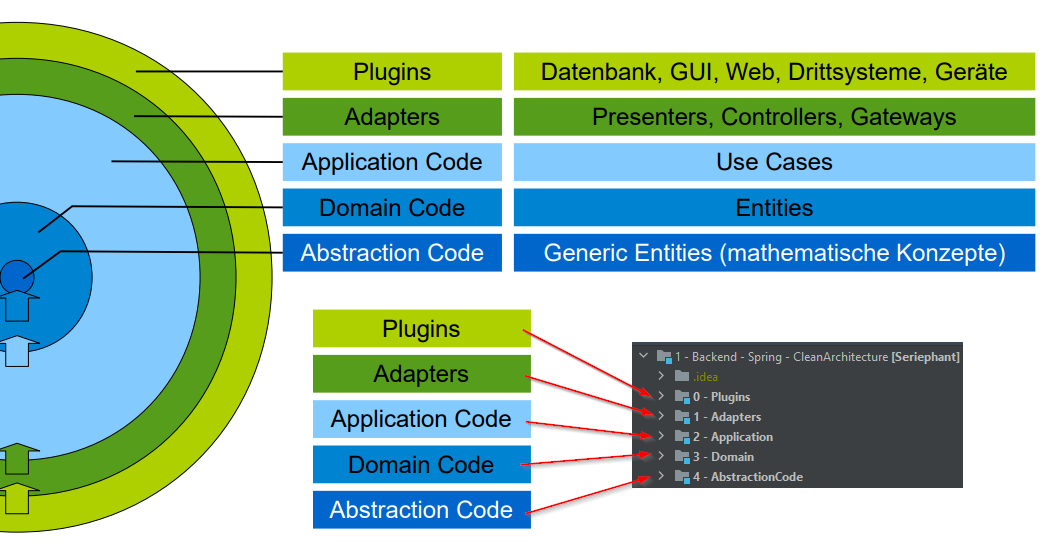
\includegraphics[width=0.95\textwidth]{zfiles/Bilder/schichten.png}

    \section{Schichtenarchitektur}
     Das Projekt soll sich an der Schichtenarchitektur orientieren. Hierbei sollen die einzelnen Module die einzelnen Schichten darstellen. Der Grund für die Benutzung einzelner Schichten ist die fachliche Unabhängigkeit der Anwendung von der sonstigen Infrastruktur. Dadurch können die einzelnen Teile leichter wiederverwendet, getestet und weiterentwickelt werden. Es ist auch leichter, einzelne Komponenten der Infrastruktur auszutauschen.
    
        \subsection{Abstraction - Schicht}
    	Diese Schicht stellt den Kern der Applikation dar. Hier werden Fundamente, oft durch die verwendete Programmiersprache geschaffen. Ein Beispiel hierfür ist die Implementierung des \hk{Strings} in Java, welche in der Spring Boot Anwendung verwendet wird.
    		\subsubsection{Implementierung im Projekt}
    		Diese Schicht wird durch Spring Boot, welches auf Java aufbaut, implementiert. 
    	
    	\subsection{Domain - Schicht}
    	In der Domain Schicht liegen die Business Objekte der Anwendung. Hier werden unternehmensweite Geschäftslogiken implementiert.
    		\subsubsection{Implementierung im Projekt}
    		In dieser Schicht liegen die Domänenobjekte, das heißt die Entities (\cref{1.entities}), Value Objects (\cref{1.vo}), Aggregates (\cref{1.aggregate}) und Repositories (\cref{1.repo}).
    	
    	\subsection{Application - Schicht}
    	In der Applikationsschicht liegen die Services, welche die Use-Cases implementieren.
    		\subsubsection{Implementierung im Projekt}
    		Die Use-Cases wurden in dieser Schicht implementiert, da sie über die Verantwortlichkeit einer einzelnen Entität hinausgehen. Diese Logiken und Prozesse wurden in sogenannte Services ausgelagert.
    	
    	\subsection{Adapters - Schicht}
    	In der Adapterschicht erfolgt die Umwandlung von Business-Objekten (interne Objekte) in Transferobjekten (externe Objekte).
    		\subsubsection{Implementierung im Projekt}
    		Hierzu werden Mapper verwendet, welche eine einfache Konvertierung von DTOs zu Entitäten und umgekehrt zulassen.
    		
    	\subsection{Plugins - Schicht}
    	In der Plugin-Schicht werden Frameworks verwendet. Diese unterstützen bestimmte Programmfunktionen, ohne diese selbst zu entwickeln und somit den selbst geschriebenen Code zu minimieren.
    	    \subsubsection{Implementierung im Projekt}
    	    In diesem Projekt sind mehrere Frameworks im Einsatz. \\
    	    \begin{itemize}
    	        \item Persistierungsframework $\rightarrow$ Hibernate
    	        \item Debug-SQL-Console $\rightarrow$ H2 Console
    	        \item API-Dokumentation \& Tests $\rightarrow$ Swagger
    	    \end{itemize}

    \section{Frontend}
    Im Frontend mussten keine Prinzipien der Clean Architecture verwendet werden. Hier kommt React zum Einsatz, um die visuelle Darstellung der Use-Cases zu implementieren.
	\ifthenelse{\boolean{DEBUG}}{}{\cleardoublepage}
	
	%%%%%%%%%%%%%%%%%%%%%%%%%%%%%%%%%%%%%%%%%%%%%%%%%%%%%%%%%%%%%%%%%%%%%%%%%%%%%%%
%% Descr:       Vorlage für Berichte der DHBW-Karlsruhe
%% Author:      Prof. Dr. Jürgen Vollmer, vollmer@dhbw-karlsruhe.de
%% Modified :	Kristin Agne, TINF19B4
%% -*- coding: utf-8 -*-
%%%%%%%%%%%%%%%%%%%%%%%%%%%%%%%%%%%%%%%%%%%%%%%%%%%%%%%%%%%%%%%%%%%%%%%%%%%%%%%

\chapter{Programming Principles}

\section{SOLID}
SOLID steht für fünf Prinzipien, die im Folgenden betrachtet werden.

    \subsection{Single Responsibility Principle}
    
        \subsubsection{Analyse}
        Das Prinzip wird bei den RepositoryInterface Klassen eingesetzt. Hierbei hat jedes RepositoryInterface nur eine genau definierte Funktion. Diese Funktion ist die Anbindung an die Datenbank.
        
        \subsubsection{Begründung}
        Der Grund dafür ist, dass eine Klasse, Methode, etc. nur eine Zuständigkeit haben soll. Es kapselt so die Zuständigkeit, diese sind klar definiert, da jede Klasse etc. nur einen Nutzen hat. Das führt dazu, dass Änderungen der Software nur zu Änderungen in einem eingegrenzten Bereich führen.

    \subsection{Open Closed Principle}
    
        \subsubsection{Analyse}
        Hierbei geht es darum, dass Klassen einfach erweiterbar sind, ohne sie grundsätzlich zu ändern. In dem Projekt kommt dieses Prinzip zum Beispiel in den Application Service Klassen oder den Controller Klassen zum Einsatz. Hierbei kann der Controller um einen Endpunkt erweitert werden, ohne dass die Klasse grundlegend modifiziert werden muss. Auch bei den Service Klassen trifft dies zu.
        
        \subsubsection{Begründung}
        Der Grund für die Benutzung dieses Prinzips ist, dass eine Erweiterung an Methoden oft vorkommt. Wenn man jedes Mal die Klasse von Grund auf ändern müsste, wäre das sehr aufwendig. Durch das Open Closed Principle kann man neue Methoden ohne großen Aufwand hinzufügen.

    \subsection{Liskov Substitution Principle}
        Unter dem Liskov Substitution Principle wird zusammengefasst, dass eine Instanz einer Klasse durch eine Instanz einer anderen Klasse, die entweder von dieser Klasse erbt oder das gleiche Interface erweitert, ersetzt werden kann. Hierbei darf es nicht zu einem logischen Bruch innerhalb der Anwendung kommen. In diesem Projekt gibt es zwar keine Vererbung, aber es wurden Interfaces benutzt. Dieses Prinzip kommt also bei den Repository Interfaces zum Einsatz. Die Bridge Klassen (z.B. GenreBridge) implementieren hierbei das Repository Interface und jede Instanz der Bridge Klasse kann durch eine Instanz ersetzt werden, die das gleiche Interface implementiert. Dies wird mit dem Liskov Substitution Principle umgesetzt, um die implementierte Logik in der Bridge Klasse einfach austauschen zu können, ohne alle Klassen anpassen zu müssen, die von den Repository Interfaces abhängig sind (wie die Application Services).

    \subsection{Interface Segregation Principle}
    
        \subsubsection{Analyse}
        Das Interface Segregation Principle wurde in den Repository Interfaces verwendet. Hierbei wurden keine unnötigen Schnittstellenteile implementiert.
        
        \subsubsection{Begründung}
        Der Grund hierfür ist, dass Schnittstellen so kleiner sind und nur verwendete Methoden zwingend implementiert werden müssen. Dadurch wird die Wartbarkeit erheblich verbessert und der Code wird kompakter und besser wiederverwendbar. Die implementierten Klassen gewinnen so an Übersichtlichkeit, fachlich zusammengehöriges Verhalten wird so gruppiert und die Modularität wird dadurch verbessert.

\subsection{Dependency Inversion Principle}

        \subsubsection{Analyse}
        Das Dependency Inversion Principle kommt vor allem bei objektorientierten Entwürfen zum Einsatz und besagt, dass höhere Module nicht von niedrigeren Modulen abhängen sollen. Die einzelnen Module stellen hierbei verschiedenen Ebenen dar. Die Ebenen haben verschiedene Ordnungen, und sind abhängig voneinander. In diesem Projekt ist die niedrigste Ebene die Plugin-Schicht (siehe \cref{cleanArchitecture}). Module niedriger Ebenen sind immer von Modulen höherer Ebenen abhängig, da Module niedrigerer Ebenen die Vorgänge der höheren Ebene spezifizieren.
        
        \subsubsection{Begründung}
        Der Grund, warum man die verschiedenen Ebenen in Module aufteilt und somit eine Abhängigkeit von niedrigen zu höheren Ebenen realisiert, ist, dass man so dem Prinzip der Hierarchie nicht widersprechen kann. Des Weiteren wird so die Vorstellung der Clean Architecture zwangsweise umgesetzt und Veränderungen in der Architektur oder des Design sind leicht umsetzbar. So wird auch die Komplexität des gesamten Projekts verringert.

\section{GRASP}
GRASP steht für General Responsibility Assignment Software Patterns. Darunter werden neun Muster verstanden, welche im Folgenden näher betrachtet werden.

	\subsection{Low Coupling and High Cohesion (Service und Controller)}
	Im Folgenden wird die Betrachtung von Low Coupling und High Cohesion in den Services und Controllern betrachtet.
		\subsubsection{Low Coupling}
			\myparagraph{Analyse}
			Bei dem Prinzip Low Coupling geht es um die Minimierung der Abhängigkeiten einer Klasse von der Umgebung. Hierbei sollten die einzelnen Klassen und Objekte möglichst wenig untereinander vernetzt sein, sodass die Abhängigkeiten so gering wie möglich gehalten sind. Dieses Prinzip wurde in einigen ApplicationServices umgesetzt, aber nicht in allen. Der ActorApplicationService oder der GenreApplicationService sind jeweils nur von einem Repository, von dem ApplicationRepository bzw. dem GenreRepository abhängig. Hier ist das Prinzip des Low Coupling umgestezt. Im Gegensatz dazu wurde das Prinzip im EpisodeApplicationService nicht umgesetzt, da hier eine Abhängigkeit zu vier Repositories besteht. Hier spricht man von High Coupling.
			
			\myparagraph{Begründung}
			Der Grund für das Einsetzen von Low Coupling ist die leichte Anpassbarkeit. Durch die geringen Abhängikeiten können ActorApplicationService und GenreApllication im Gegensatz zum EpisodeApllicationService leicht angepasst werden. Auch die Verständlichkeit der beiden Klassen mit Low Coupling ist einfacher und man kann die beiden Klassen besser wieder verwenden. Zusätzlich ist das Testen von Klassen mit Low Coupling einfacher, da man nur auf wenige Abhängigkeiten achten muss.
		
		\subsubsection{High Cohesion}
			\myparagraph{Analyse}
			Bei dem Prinzip High Cohesion geht es um die Vermeidung von verschiedenen Verantwortlichkeiten bzw. Aufgaben innerhalb einer Klasse. Hierbei wird betrachtet, inwieweit die Objekte und Attribute einer Klasse zusammenarbeiten und wie viel sie über andere Objekte wissen müssen. Im Projekt wurde dieses Prinzip zum Beispiel in den Controllern umgesetzt. Hierbei bekommen die Controller eine Anzahl von Parametern und eine Methode, und sie verarbeiten diese Daten mit Hilfe des Services. Dabei haben die Controller nur eine Art von Verantwortlichkeit und somit ist das Prinzip der hohen Kohäsion hier umgesetzt.
			
			\myparagraph{Begründung}
			Der Grund für die Umsetzung des Prinzips ist, dass man so die Übersichtlichkeit der Klasse deutlich verbessert und die Komplexität minimiert.
			
		\subsubsection{Zusammenhang Low Coupling und High Cohesion}
		Diese zwei Prinzipien stehen bei den Service und Controller Klassen in negativer Korrelation zueinander. Je mehr Verantwortlichkeiten man in andere Klassen auslagert, desto höher wird die Cohesion zwischen den Klassen und desto höher wird auch die Abhängigkeit. High Cohesion geht also mit High Coupling einher, Low Coupling und High Cohesion voll umzusetzen ist schwierig, man sollte ein Mittel finden, bei dem das Coupling möglichst low und die Cohasion möglichst high ist.
	
	\subsection{Loose Coupling und High Cohesion (Domain)}
	Im Bereich der Domäne verhält sich die Verbindung zwischen Low Coupling und High Cohesion synchron.
	
		\subsubsection{Loose Coupling}
		
		\myparagraph{Analyse}
		Bei dem Prinzip Loose Coupling geht es um die Minimierung der Abhängigkeiten einer Klasse von der Umgebung. Betrachtet man die Klassen innerhalb der Domäne, sieht man, dass hier Tight Coupling ist. Da die beispielsweise die Klasse Genre eine List<Serie> und jede Serie ein Genre Objekt hat, sind die beiden Klassen gekoppelt. 
		
		\myparagraph{Begründung}
		Der Grund für diese Umsetzung und die hohe Kopplung ist, wie in Spring die Entities angelegt wurden und wie mit deren Beziehungen umgegangen wird. Hierbei werden komplette Objekte anstelle von ihren Id's referenziert.
		
		\subsubsection{High Cohesion}
		
		\myparagraph{Analyse}
		Bei dem Prinzip High Cohesion geht es um die Vermeidung von verschiedenen Verantwortlichkeiten bzw. Aufgaben innerhalb einer Klasse. Innerhalb der Domäne hätte man aufgrund von Tight Coupling eigentlich eine Low Cohesion, da durch die hohe Abhängigkeit von der Genre und Serie Klasse Funktionen gegenseitig übernommen werden müssten. Jedoch ist dies durch Spring nicht der Fall, weil das Genre theoretisch nur in der Serie gespeichert ist und beim Persistieren die List<Serie> in der Genre Klasse von Spring automatisch geupdatet wird.
		
		\myparagraph{Begründung}
		Auch hierfür ist der Grund Verbesserung der Übersichtlichkeit der Klasse sowie die Minimierung der Komplexität.
		
		\subsubsection{Zusammenhang Loose Coupling und High Cohesion}
		Normalerweise stehen Loose Coupling und High Cohesion in der Domäne synchron in Beziehung, da bei einer geringen Anzahl von Abhängikeit auch eine hohe Kohäsion umgesetzt wird. Allerdings ist durch Spring und die Verwendung von Hibernate hier Tight Coupling umgesetzt, und trotzdem ist noch eine hohe Kohäsion vorhanden.

    \subsection{Creator}
    Unter dem Erzeuger-Prinzip versteht man das Prinzip, dass eine Instanz einer Klasse nur von einem Experten A erzeugt wird. In diesem Projekt findet das Creator-Pattern den Einsatz beispielweise im RatingApplicationService. Dieser sammelt die benötigten Initialisierungsdaten und instanziiert dann ein RatingAverage. Man könnte sagen, der RatingApplicationService ist der Experte A für die Erzeugung eines Rating Average.
    
    \subsection{Controller}
    Das Controller-Pattern findet in dem Projekt in den Controllern in der Plugins-Schicht Anwendung. Sie sind dafür zuständig, um die Benutzereingaben zu empfangen und zu verarbeiten. Ein Request wird mit Parametern von einem Controller entgegengenommen und von diesem wird die entsprechende Methode aufgerufen.
    
    \subsection{Indirection}
    Das Indirection Pattern wird verwendet, um Low Coupling umzusetzen. Es wird ein sogenannter Vermittler zwischen Client und Server eingesetzt. In diesem Projekt findet dieses Pattern keinen Einsatz, da die Leistungsfähigkeit so vermindert wird.
    
    \subsection{Information Expert}
    Bei dem Information Expert Pattern geht es darum, dass eine Klasse nur genau die Informationen kennt, die sie auch benötigt, um ihrer Verantwortung gerecht zu werden. Das heißt, eine Aufgabe wird immer von der Klasse übernommen, die das meiste benötigte Wissen besitzt. Dieses Pattern fördert high cohesion. Umgesetzt wird dieses Pattern in den Entitäten und Repositories. Die Entitäten kapseln das Wissen, sodass nur mit Gettern und Settern darauf zugegriffen werden kann. Bei den Repositories übernimmt immer genau das Repository die Aufgabe, welches das meiste Wissen hat.
    
    \subsection{Polymorphism}
    Das Polymorphism-Pattern wird in diesem Projekt nicht umgesetzt, da es keine Anwendungsfälle (beispielsweise Vererbung oder verschiedene Ausprägungen einer Interface Methode) in diesem Projekt gibt.
    
    \subsection{Protected Variations}
    Das Protected Variations Pattern wird in diesem Projekt durch die Repository Interfaces in der Domänenschicht, die in der Plugins Schicht implementiert werden, umgesetzt. Dadurch wird die eigentliche Implementierung in der Plugins Schicht über die Interfaces verschleiert. So hat eine Veränderung an der Implementierung keine Auswirkung auf das restliche System.
    
    \subsection{Pure Fabrication}
    Das Pure Fabrication Pattern stellt Klassen dar, die in der Domäne nicht existieren. In diesen Klassen werden beispielsweise Methoden ausgelagert und die Klassen werden als Erfindung bezeichnet, da sie nichts Reales aus der Domänenschicht repräsentieren. Dieses Pattern wird zur Unterstützung von high cohesion und low coupling eingesetzt. In diesem Projekt wird Pure Fabrication durch die Data Transfer Objects (DTO) in der Adapter Schicht umgesetzt. Durch diese Klassen wird beispielsweise das Frontend von der Domäne entkoppelt. Eine Anpassung der Domäne führt nicht zwingend zu einer Anpassung des Frontends und umgekehrt.

\section{DRY}
Das Prinzip DRY bedeutet \hk{Don't Repeat yourself}. Hierbei handelt es sich um ein Prinzip des Clean Code, damit Codeabschnitte nicht wiederholt, sondern stattdessen ausgelagert und wiederverwendet werden.

    \subsection{Analyse}
    Diese Prinzip ist ein grundlegendes Prinzip und wurde prinzipiell in dem gesamten Projekt umgesetzt. Im \cref{refactoring} sieht man die Extraktion von Teilen einer Methode in einzelne neue Methoden. Diese neuen Methoden werden anschließend auch von anderen Methoden benutzt, wodurch eine Wiederholung vermieden wird.
    
    \subsection{Begründung}
    Diese Prinzip hat mehrere Vorteile, da man so weniger Code schreiben muss und sich somit Zeit spart. Außerdem nimmt die Übersichtlichkeit enorm zu, wenn man gleiche Teile in Methoden auslagert und mehrfach verwendet. Nicht nur die Übersichtlichkeit, sondern auch die Verständlichkeit und Fehleranfälligkeit des Codes wird so verbessert. Des Weiteren wird die Wartbarkeit vereinfacht, weil man so bei Logikfehlern oder Veränderungen nur eine Methode und nicht alle Codestellen anpassen muss.
	\ifthenelse{\boolean{DEBUG}}{}{\cleardoublepage}
	
	%%%%%%%%%%%%%%%%%%%%%%%%%%%%%%%%%%%%%%%%%%%%%%%%%%%%%%%%%%%%%%%%%%%%%%%%%%%%%%%
%% Descr:       Vorlage für Berichte der DHBW-Karlsruhe
%% Author:      Prof. Dr. Jürgen Vollmer, vollmer@dhbw-karlsruhe.de
%% Modified :	Nico Holzhäuser, TINF19B4
%% -*- coding: utf-8 -*-
%%%%%%%%%%%%%%%%%%%%%%%%%%%%%%%%%%%%%%%%%%%%%%%%%%%%%%%%%%%%%%%%%%%%%%%%%%%%%%%

\chapter{Refactoring}
\label{refactoring}

\section{Identifizieren von Codesmells}

    \subsection{Code Smell 1}
    Hierbei handelt es sich um den Code Smell "Long method". Methoden sollen kurz und übersichtlich sein, die folgende Methode ist aber lang und verschachtelt.
    
    \begin{figure}[h]
	    \centering
        \shadowimage[width=0.95\textwidth]{zfiles/Bilder/long_method_old.png}
	    %\shadowimage[height=250px]{./zfiles/Bilder/cleanArchitecture.png}
	    \caption{Code Smell "Long method" before fix}
	    \label{a.2.cleanArchitecture}
    \end{figure}
    
    
        \subsubsection{Begründung}
        Die Methode ist 20 Zeilen lang und sehr verschachtelt. Dadurch ist es schwer, auf den ersten Blick zu erkennen, was die Methode macht. Auch ist die Methode nicht übersichtlich.

        \subsubsection{Fix}
        Durch das Auslagern von einzelnen Teilen der Methode wird klarer, was wo passiert und warum. In meinem Projekt gab es einige weitere lange Methoden, die sehr unübersichtlich waren. Durch die Umstrukturierung von einer langen Methode in mehrere kurze werden die einzelnen Teile der Methode übersichtlicher und sind leichter verständlich.
    
        \begin{figure}[h]
	        \centering
            \shadowimage[width=0.8\textwidth]{zfiles/Bilder/long_method_fix.png}
	        %\shadowimage[height=250px]{./zfiles/Bilder/cleanArchitecture.png}
	        \caption{Code Smell "Long method" before fix}
	        \label{a.2.cleanArchitecture}
        \end{figure}
    
    

    \subsection{Code Smell 2}
    Bei diesem Code Smell geht es darum, dass ungenutze private Variablen entfernt werden.
    \begin{figure}[h]
	    \centering
        \shadowimage[width=0.95\textwidth]{zfiles/Bilder/unused_variable_old.png}
	    %\shadowimage[height=250px]{./zfiles/Bilder/cleanArchitecture.png}
	    \caption{Code Smell "Long method" before fix}
	    \label{a.2.cleanArchitecture}
    \end{figure}

        \subsubsection{Begründung}
        Wenn eine private Variable oder ein Import in der Klasse nicht benutzt werden, sind diese unnötig und verschlechtern nur die Übersichtlichkeit und Fehleranfälligkeit des Codes. 

        \subsubsection{Fix}
        Für den Fix wurden hierbei einfach die unbenutze private Variablendeklaration entfernt und auch die Zuweisung aus dem Konstruktor wurde entfernt.
        \begin{figure}[h]
	        \centering
            \shadowimage[width=0.8\textwidth]{zfiles/Bilder/unused_variable_fix.png}
	        %\shadowimage[height=250px]{./zfiles/Bilder/cleanArchitecture.png}
	        \caption{Code Smell "Long method" before fix}
	        \label{a.2.cleanArchitecture}
        \end{figure}

	\ifthenelse{\boolean{DEBUG}}{}{\cleardoublepage}
	
	\ifthenelse{\boolean{TRENNSTRICHE}}{\addtocontents{toc}{\protect\mbox{}\protect\hrulefill\par}}{}
	%%%%%%%%%%%%%%%%%%%%%%%%%%%%%%%%%%%%%%%%%%%%%%%%%%%%%%%%%%%%%%%%%%%%%%%%%%%%%%%
%% Descr:       Vorlage für Berichte der DHBW-Karlsruhe
%% Author:      Prof. Dr. Jürgen Vollmer, vollmer@dhbw-karlsruhe.de
%% Modified :	Nico Holzhäuser, TINF19B4
%% -*- coding: utf-8 -*-
%%%%%%%%%%%%%%%%%%%%%%%%%%%%%%%%%%%%%%%%%%%%%%%%%%%%%%%%%%%%%%%%%%%%%%%%%%%%%%%

\chapter{Entwurfsmuster}
Das Objektmuster \hk{Bridge Pattern} kam in diesem Projekt zum Einsatz. 

\section{Begründung des Einsatzes}
Dieses Entwurfsmuster wurde eingesetzt, da so eine Entkopplung von Domänenmodell und Persistierungslogik gelingt. Die Trennung von Domänenmodell und Persistierungslogik ist Teil von Clean Architecture, da so die Persistierung leicht ausgetauscht werden kann. Hierbei erfolgt die Implementierung in Form eines Interfaces im Domänenmodell, welches von einer Bridge mit Hilfe eines ORM-Plugins in der Plugins-Schicht umgesetzt wird.

\section{\ac{UML} Vorher}
Im Folgenden sieht man das \ac{UML} Diagramm vor der Verwendung des Bridge Patterns. Hierbei hat das Repository als Child von einem JPA Repository direkt auf die Datenbank zugegriffen. Die Persistierungslogik war so nicht getrennt und konnte nur mit mehreren Anpassungen ausgetauscht werden.

        \begin{figure}[H]
	        \centering
            \shadowimage[width=0.8\textwidth]{zfiles/Bilder/uml_vorher.png}
	        \caption{UML Diagramm ohne Benutzung des Bridge Pattern}
        \end{figure}

\section{\ac{UML} Nachher}
Beim \ac{UML} Diagramm nach der Verwendung des Bridge Patterns sieht man, das mehr Klassen beteiligt sind. Zwischen Repository und JPARepository sind zum einen die Bridge sowie das Spring DataRepository dazwischen. Dadurch wird die Persistierung nicht mehr direkt, sondern über die Bridge durchgeführt.

        \begin{figure}[H]
	        \centering
            \shadowimage[width=0.8\textwidth]{zfiles/Bilder/uml_nachher.png}
	        \caption{UML Diagramm mit Benutzung des Bridge Pattern}
        \end{figure}
	%Trennlinie fürs ToC beim letzten Kapitel!
	
	\ifthenelse{\boolean{DEBUG}}{}{\cleardoublepage}
	
	%—————————————————————————————————————————————————————————————————————————
	%								Anhang
	%—————————————————————————————————————————————————————————————————————————
	%Anhang mit großen römischen Zahlen
%	\pagenumbering{Roman}
%	\appendix
%	%======================================================================
%	
%	                _                       
%	    /\         | |                      
%	   /  \   _ __ | |__   __ _ _ __   __ _ 
%	  / /\ \ | '_ \| '_ \ / _` | '_ \ / _` |
%	 / ____ \| | | | | | | (_| | | | | (_| |
%	/_/    \_\_| |_|_| |_|\__,_|_| |_|\__, |
%								       __/ |
%									  |___/ 
%
%----------------------------------------------------------------------
% Descripton : Appendix Main File to Compose differtend Appendix
%======================================================================

\pagestyle{plain}

\chapter{Anhang}

%Fixxing Lstlisting and formular
\addtocontents{lol}{\protect\addvspace{10pt}}
\addtocontents{for}{\protect\addvspace{10pt}}

%======================================================================
%	
%	                _                       
%	    /\         | |                      
%	   /  \   _ __ | |__   __ _ _ __   __ _ 
%	  / /\ \ | '_ \| '_ \ / _` | '_ \ / _` |
%	 / ____ \| | | | | | | (_| | | | | (_| |
%	/_/    \_\_| |_|_| |_|\__,_|_| |_|\__, |
%								       __/ |
%									  |___/ 
%
%----------------------------------------------------------------------
% Descripton : Appendix 1
%======================================================================

\section{Ubiquitous Language} \label{a.1.pic}
\begin{figure}[h]
	\centering
	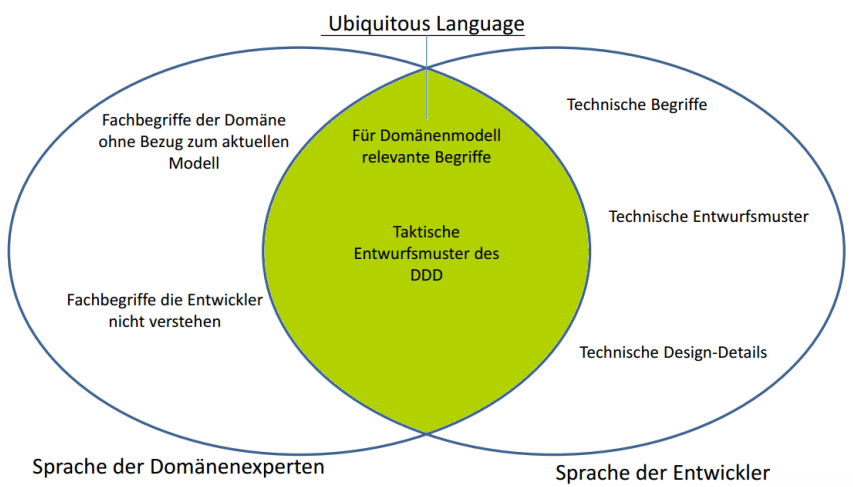
\includegraphics[height=250px]{./appendix/filesONLYForAppendix/Images/ul.png}
	\caption{Gemeinsame Projektsprache von Domänenexperten und Entwickler}
	\label{Löwe}
\end{figure}

\newpage


%======================================================================
%	
%	                _                       
%	    /\         | |                      
%	   /  \   _ __ | |__   __ _ _ __   __ _ 
%	  / /\ \ | '_ \| '_ \ / _` | '_ \ / _` |
%	 / ____ \| | | | | | | (_| | | | | (_| |
%	/_/    \_\_| |_|_| |_|\__,_|_| |_|\__, |
%								       __/ |
%									  |___/ 
%
%----------------------------------------------------------------------
% Descripton : Appendix 2
%======================================================================
%======================================================================
%	
%	                _                       
%	    /\         | |                      
%	   /  \   _ __ | |__   __ _ _ __   __ _ 
%	  / /\ \ | '_ \| '_ \ / _` | '_ \ / _` |
%	 / ____ \| | | | | | | (_| | | | | (_| |
%	/_/    \_\_| |_|_| |_|\__,_|_| |_|\__, |
%								       __/ |
%									  |___/ 
%
%----------------------------------------------------------------------
% Descripton : Appendix 3
%======================================================================
%======================================================================
%	
%	                _                       
%	    /\         | |                      
%	   /  \   _ __ | |__   __ _ _ __   __ _ 
%	  / /\ \ | '_ \| '_ \ / _` | '_ \ / _` |
%	 / ____ \| | | | | | | (_| | | | | (_| |
%	/_/    \_\_| |_|_| |_|\__,_|_| |_|\__, |
%								       __/ |
%									  |___/ 
%
%----------------------------------------------------------------------
% Descripton : Appendix 4
%======================================================================
%======================================================================
%	
%	                _                       
%	    /\         | |                      
%	   /  \   _ __ | |__   __ _ _ __   __ _ 
%	  / /\ \ | '_ \| '_ \ / _` | '_ \ / _` |
%	 / ____ \| | | | | | | (_| | | | | (_| |
%	/_/    \_\_| |_|_| |_|\__,_|_| |_|\__, |
%								       __/ |
%									  |___/ 
%
%----------------------------------------------------------------------
% Descripton : Appendix 5
%======================================================================
%	\cleardoublepage
%	\ifthenelse{\boolean{DEBUG}}{}{\cleardoublepage}
	
	%—————————————————————————————————————————————————————————————————————————
	%						Literaturverzeichnis
	%—————————————————————————————————————————————————————————————————————————
	\renewcommand\bibname{Literaturverzeichnis \\ \vspace{10mm} \normalsize{} Alle Quellen sind zusätzlich im Ordner \HREF{./Quellensicherung}{Quellensicherung} gespeichert ! \vspace{-2cm}}
	\phantomsection
	\addcontentsline{toc}{chapter}{Literaturverzeichnis}
	\printbibliography
	\ifthenelse{\boolean{DEBUG}}{}{\cleardoublepage}
	
\end{document}